\documentclass[a4paper,12pt]{ctexart}
% \usepackage{xeCJK}
\usepackage{amsmath}
\usepackage{amsfonts}
\usepackage{float}
\usepackage{enumerate}
\usepackage{graphicx}
\usepackage{tikz}
\usepackage{pgfplots}
\usepackage[scale=0.8]{geometry}
\usepackage[hidelinks]{hyperref}
\title{经济学综合第二次作业}
\author{董晨阳 2201211201}
\date{\today}
\begin{document}
\maketitle
\section{税收政策:预期与非预期,永久与暂时}
\subsection*{a}
政府征税导致家庭面对的真实利率变为$(1-\tau)f'(k(t))$,消费的欧拉方程变为
\begin{equation}
    \frac{\dot c}{c}=\frac{(1-\tau)f'(k)-\rho-\theta g}{\theta}
\end{equation}
因此$\dot c=0$向左移动,$\dot k=0$无变化
\subsection*{b}\label{sec:b}
$c^*$与$k^*$均减小
\subsection*{c}
如果采用政府购买的方式,则在(\nameref{sec:b})基础上会进一步对$\dot k=0$产生影响
\begin{equation}
    \dot k=f(k_t)-c_t-(\tau r+n+g)k_t
\end{equation}
使得$\dot k=0$向内移动,使得相较于(\nameref{sec:b}),$k^*$不变但$c^*$减小
\subsection*{d}
从$t=0$到$t1$时刻之间,如(\nameref{sec:g})中所说,$c$跃迁后资本存量无法维持,$k$会持续减小。但此时经济处于原$\dot c=0$的左侧,消费先增加,直到到达鞍点路径上。
\subsection*{e}
若要求经济到达新的平衡增长路径,则在开征税收时经济必须处于新的鞍点路径。在$t_1$时刻,$\dot c=0$左移,但消费$c$不会出现非连续变化,否则不是家庭最优结果
\subsection*{f}
在$t_1$时刻之后,消费$c$和$k^*$如果尚未达到均衡点,则均会减小且连续;如果已经达到均衡点,则将维持不变,但不可能低于均衡点
\subsection*{g}\label{sec:g}
在$0$时刻,消费$c$会出现非连续变化。如若立即实行该政策,则消费$c$会出现迅速增加后逐步减少。但该政策为一段时间后的执行,因而当前家庭消费会增加,但是没有立即执行增加那么多。
\subsection*{h}\label{sec:h}
如图所示
\begin{figure}[H]
    \begin{minipage}{0.48\linewidth}
        \centering
        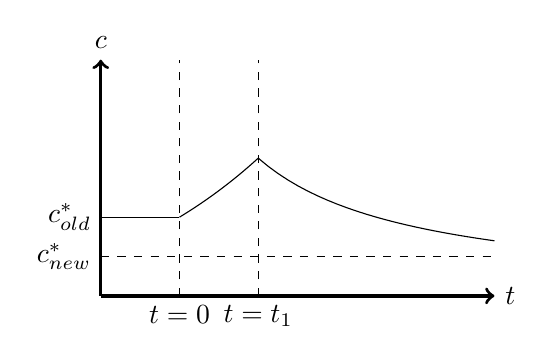
\begin{tikzpicture}
            \draw[->,very thick] (0,0) -- (5,0) node[right] {$t$};
            \draw[->,very thick] (0,0) -- (0,3) node[above] {$c$};
            \draw (0,1)--(1,1);
            \draw[domain=1:2] plot (\x,1.5^\x-0.5);
            \draw[domain=2:5] plot (\x,3.5/\x);
            \draw[dashed] (1,0)--(1,3);
            \draw[dashed] (0,0.5)--(5,0.5);
            % \draw (4,0.5)--(5,0.5);
            \draw[dashed] (2,0)--(2,3);
            \node[below] at (1,0){$t=0$};
            \node[below] at (2,0){$t=t_1$};
            \node[left] at (0,1){$c^*_{old}$};
            \node[left] at (0,0.5){$c^*_{new}$};
        \end{tikzpicture}
    \end{minipage}
    \begin{minipage}{0.48\linewidth}
        \centering
        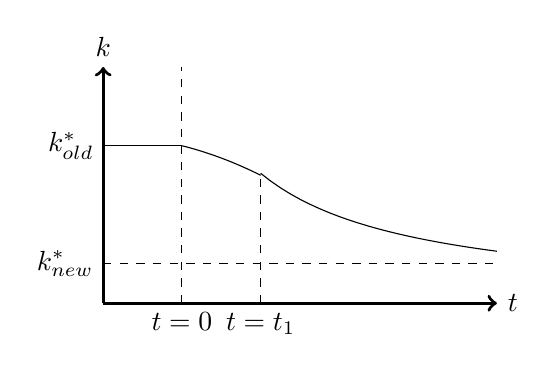
\begin{tikzpicture}
            \draw[->,very thick] (0,0) -- (5,0) node[right] {$t$};
            \draw[->,very thick] (0,0) -- (0,3) node[above] {$k$};
            \draw (0,2)--(1,2);
            \draw[domain=1:2] plot (\x,2.125-\x^2/8);
            \draw[domain=2:5] plot (\x,3.3/\x);
            \draw[dashed] (1,0)--(1,3);
            \draw[dashed] (0,0.5)--(5,0.5);
            \draw[dashed] (2,0)--(2,1.625);
            \node[below] at (1,0){$t=0$};
            \node[below] at (2,0){$t=t_1$};
            \node[left] at (0,2){$k^*_{old}$};
            \node[left] at (0,0.5){$k^*_{new}$};
        \end{tikzpicture}
    \end{minipage}
\end{figure}
\subsection*{i}\label{sec:i}
消费$c$在$t_1$时不会不连续变化,因为家庭已经事先知道税收终结的时间,消费$c$的不连续变化违反家庭跨期优化的消费平滑要求,因此在时间$t_1$的时刻经济必须处于旧的鞍点路径的某个位置。

在$t=0$到$t=t_1$之间,$\dot c= 0$位于原来位置的左方。为了回到均衡点, $t=0$时$c$必须向上跳跃,此后$k$和$c$都开始下降。经济最终穿过 $\dot k=0$ 曲线,$K$开始增加。这是因为家庭预期资本税将退出,又开始愿意积累资本了。 $t_1$时到达旧的左下方鞍点路径上。在$t_1$ 之后,恢复到原来的 $\dot c=0$,经济沿旧的鞍点路径上移,最终回到旧的平衡增长路径。
\subsection*{j}
同(\nameref{sec:i})消费$c$在$t_1$和$t_2$不会不连续变化。
为使经济回到平衡增长路径,经济必须在时间 $t_2$ 的时刻处于旧的鞍点路径的某个位置。

$t=0$时,消费$c$会跳跃增加而$k$不变,$t=0$之后$k$减小使得经济位于$c=0$左侧,经济体向左上移动。

$t_1$时刻, $\dot c=0$左移,经济仍然位于 $\dot k=0$上方和$\dot c=0$曲线的右方,$k$继续下降, $c$停止增加而开始下降。

经济最终穿过$\dot k=0$曲线,$k$开始增加。在资本税实际退出之前,家庭又开始积累资本。 在征税结束$t_2$时刻经济体正好处于旧的鞍点路径上,此后$\dot c=0$回到原来位置上,经济沿鞍点路径上移,最终到达旧的平衡增长路径。
\end{document}
